%=======================================================================
% Journal manuscript (SCI / Scopus Q2 target)
% Compile on Overleaf: menu -> pdfLaTeX, run twice + BibTeX.
% Class: IEEEtran (journal mode). Overleaf has IEEEtran + all packages.
%
% RED [PLACEHOLDER] text = numbers you must fill in AFTER running the
% research/ pipeline. Search the file for "PLACEHOLDER" and "\ph".
%=======================================================================
\documentclass[journal]{IEEEtran}

\usepackage{amsmath,amssymb}
\usepackage{graphicx}
\usepackage{booktabs}
\usepackage{multirow}
\usepackage{url}
\usepackage[table]{xcolor}
\usepackage{tikz}
\usetikzlibrary{shapes.geometric,arrows.meta,positioning,calc}
\usepackage{algorithm}
\usepackage{algpseudocode}
\usepackage[hidelinks]{hyperref}

% Placeholder macro: renders in red so unfilled numbers are obvious.
\newcommand{\ph}[1]{{\color{red}\textbf{[#1]}}}

\begin{document}

\title{A Deployable Hybrid Rule--Transformer Web Application Firewall with
Inline Blocking and False-Positive-Controlled Decision Fusion}

\author{%
\IEEEauthorblockN{Rhenius Abraham\IEEEauthorrefmark{1}, and Co-authors\IEEEauthorrefmark{2}}%
\thanks{\IEEEauthorrefmark{1}Department of Cyber Security Engineering,
\ph{Institution}, \ph{City}, \ph{Country}
(e-mail: rhenius1603@gmail.com).}%
\thanks{Manuscript submitted \ph{Month Year}.}%
}

\markboth{IEEE/Elsevier Manuscript, \ph{Year}}%
{Abraham \MakeLowercase{\textit{et al.}}: Deployable Hybrid Rule--Transformer WAF}

\maketitle

%-----------------------------------------------------------------------
\begin{abstract}
Web application firewalls (WAFs) are the first line of defence against
injection-style web attacks, yet the two dominant paradigms each fall short:
signature and regular-expression rule sets are brittle against obfuscation and
demand constant tuning, while recent transformer-based detectors report
near-perfect offline accuracy on benchmark corpora but are almost never
deployed in the live blocking path, leave latency unmeasured, and ignore the
operational cost of false positives. We present a deployable web application
firewall that integrates a fine-tuned transformer classifier into a transparent
inline enforcement path built on the Nginx \texttt{auth\_request} mechanism,
requiring no changes to the protected application. Detection is governed by a
four-tier decision-fusion policy that couples deterministic signatures and
anomaly rules with confidence-banded model scoring, explicitly designed to
bound false positives on legitimate application traffic. We evaluate the system
end to end on \ph{N} public datasets, including a cross-dataset protocol that
tests generalisation to an unseen traffic distribution, an ablation isolating
the transformer's contribution over the rule engine, a threshold-sensitivity
analysis of the false-positive/recall trade-off, a measured latency and
throughput characterisation of transformer inference in the inline path, and an
adversarial-evasion stress test. The hybrid configuration attains an F1 of
\ph{F1} at a false-positive rate of \ph{FPR}, retains an F1 of \ph{xF1} under
cross-dataset transfer, and adds a median inline overhead of \ph{lat}~ms per
request. These results characterise, rather than merely assert, the practical
deployability of transformer-based inline web attack detection.
\end{abstract}

\begin{IEEEkeywords}
Web application firewall, transformer, BERT, intrusion detection, inline
enforcement, decision fusion, false-positive control, adversarial robustness.
\end{IEEEkeywords}

%=======================================================================
\section{Introduction}
\IEEEPARstart{W}{eb} applications remain the most exposed surface of modern
software systems, and injection-style attacks---SQL injection, cross-site
scripting (XSS), path traversal, command injection and their encoded
variants---continue to dominate the OWASP Top Ten. The web application firewall
(WAF) is the standard mitigation: a policy-enforcing intermediary that inspects
incoming requests and blocks those judged malicious before they reach the
origin application.

For two decades the enforcement logic of production WAFs has been dominated by
signatures and regular expressions, exemplified by ModSecurity paired with the
OWASP Core Rule Set~\cite{owaspcrs}. Rule sets are fast, auditable and
deterministic, but they share a well-documented weakness: they match surface
strings, not intent. An attacker who inserts inline comments, alternates
character case, or applies successive URL encodings can express a functionally
identical payload that the rule set no longer matches, while defenders who
tighten rules to catch such variants pay in false positives on legitimate
traffic. In modern applications built around single-page front ends,
WebSocket channels and continuous polling, the volume of unusual-but-benign
request shapes makes this tuning burden acute.

Learning-based detection promises to close this gap by modelling the structure
of malicious payloads rather than enumerating their spellings. Transformer
language models~\cite{vaswani2017attention,devlin2019bert} are a natural fit:
treating an HTTP request as a token sequence lets a fine-tuned encoder capture
the contextual regularities that distinguish an injection attempt from an
ordinary parameter value. A substantial recent literature does exactly this and
reports accuracies above 99\% on the standard CSIC~2010
benchmark~\cite{wadbert2026,liu2024bertlstm,scireports2023xsssqli}.

Yet a gap separates these results from a firewall a practitioner can deploy.
Almost all of this work stops at offline classification: a model is trained and
tested on a static corpus, an accuracy is reported, and the analysis ends.
Three questions that determine whether such a detector can serve as a WAF are
left unanswered. First, \emph{deployability and cost}: what latency does
transformer inference add when it sits in the synchronous path of every
request, and what throughput can the resulting system sustain? Second,
\emph{false-positive control}: an operator does not optimise raw accuracy but
the rate at which legitimate users are wrongly blocked at a chosen operating
point---a quantity these papers rarely report. Third, \emph{generalisation}:
models trained and tested on the same synthetic corpus may not transfer to a
different traffic distribution, and evaluations that never test transfer cannot
support claims of detecting novel attacks.

This paper addresses those questions directly. We build a WAF in which a
fine-tuned transformer is not a post-hoc classifier but a component of a live
inline enforcement path, and we characterise the resulting system along exactly
the axes the offline literature omits. Our contributions are:

\begin{enumerate}
\item \textbf{A deployable inline architecture.} We integrate a transformer
classifier into a transparent enforcement path using the Nginx
\texttt{auth\_request} mechanism, so that every request is adjudicated before
proxying with no modification to the protected application
(Section~\ref{sec:arch}).
\item \textbf{A false-positive-controlled decision-fusion policy.} We define a
four-tier policy that combines deterministic signatures, anomaly rules and
confidence-banded model scoring, together with an endpoint-aware relaxation and
a fail-open safeguard, and we formalise it as an algorithm
(Section~\ref{sec:method}).
\item \textbf{An end-to-end empirical characterisation.} We report detection
quality with an emphasis on false-positive rate, an ablation isolating the
transformer's contribution over the rules, cross-dataset generalisation, a
threshold-sensitivity analysis, and measured inline latency and throughput
(Section~\ref{sec:results}).
\item \textbf{An adversarial-evasion stress test} that mutates blocked payloads
with semantics-preserving transformations and reports the resulting evasion
rate, a robustness check almost absent from prior transformer-WAF work
(Section~\ref{sec:results}).
\end{enumerate}

The remainder of the paper reviews related work
(Section~\ref{sec:related}), presents the architecture
(Section~\ref{sec:arch}), methodology (Section~\ref{sec:method}) and
experimental setup (Section~\ref{sec:setup}), reports and discusses results
(Sections~\ref{sec:results}--\ref{sec:discussion}), and concludes
(Section~\ref{sec:conclusion}).

%=======================================================================
\section{Literature Survey}
\label{sec:related}
We organise prior work into four themes and, in each, identify the limitation
that motivates our design; we draw predominantly on work from 2023 onward, with
older entries retained only where they are the canonical source (foundational
models, standard datasets). A recent comprehensive survey of transformers and
large language models for intrusion detection~\cite{kheddar2025survey} situates
this literature and reports accuracies of 85--99\% for BERT- and GPT-style
models across CSIC~2010, CICIDS2017 and UNSW-NB15, while noting that deployment
efficiency and explainability remain open. Table~\ref{tab:related} summarises the
comparison.

\subsection{Rule-based and signature WAFs}
The reference point for practical web defence is ModSecurity with the OWASP Core
Rule Set~\cite{owaspcrs}, a curated collection of signatures and scoring rules.
Such systems are transparent and fast but match syntax rather than semantics;
studies of payload obfuscation show that encoding and comment insertion defeat
them, and operators trade detection for false positives when hardening the
rules. These properties make rule sets an indispensable baseline and a natural
first tier in a layered system, but an insufficient detector on their own.

\subsection{Classical machine learning for web attack detection}
A second line of work extracts features---$n$-grams, term-frequency vectors,
handcrafted lexical statistics---from HTTP requests and applies classifiers such
as support vector machines and random forests, most often on
CSIC~2010~\cite{gimenez2010csic}. Recent studies continue this approach: web
payloads are classified into SQL injection, XSS and command injection with SVM,
random-forest and XGBoost models~\cite{payloadml2024svmrfxgb}, and enhanced
neural architectures have been proposed for precision web attack
detection~\cite{zhou2025ewebguard}. These methods run cheaply but depend on
feature engineering and tend to generalise poorly beyond their training
distribution, capturing lexical rather than contextual regularities. We include
TF--IDF support-vector and random-forest models as baselines.

\subsection{Deep learning and transformer-based detection}
Treating requests as text, deep models---CNNs, LSTMs and, increasingly,
transformer encoders---learn payload structure directly. Recent deep architectures
report near-perfect within-corpus accuracy: a novel deep model secures web
applications against XSS and SQLi with accuracies above 99\% on CSIC~2010 and
payload testbeds~\cite{scireports2024novelxsssqli}, command-injection detectors
reach comparable figures~\cite{scireports2024cmdi}, and ensembles of LSTM, GRU
and stacked autoencoders target so-called zero-day web
attacks~\cite{zeroday2025ensemble}. On the transformer side, BERT and its
relatives~\cite{devlin2019bert,liu2019roberta} have been fine-tuned for SQL
injection detection through a BERT--LSTM hybrid~\cite{liu2024bertlstm} and for
dual-channel web attack detection~\cite{wadbert2026}; BERT has been applied to
intrusion detection more broadly~\cite{yang2025bertids}, to unseen-attack
detection in software-defined networks~\cite{sdnbert2024}, and to web-server log
classification via transfer learning~\cite{prasetyo2025webserver}. Domain-adapted
encoders such as SecureBERT~\cite{aghaei2022securebert,aghaei2025securebert2}
pretrain on cybersecurity text and could, in principle, improve request
classification, though they have not been evaluated in that role, and
self-supervised HTTP embeddings have also been
proposed~\cite{http2vec2021}. The recurring limitation across this group is that
evaluation is offline: the model is not placed in an enforcement path, latency is
not reported, and false-positive behaviour at an operating point is not analysed.
Log-anomaly detectors such as LogBERT~\cite{guo2021logbert} share the
sequence-modelling idea in an adjacent setting.

\subsection{Compression, latency, datasets and adversarial evasion}
Because transformer inference is costly, a compression literature distils and
prunes these models: DistilBERT~\cite{sanh2019distilbert} and
TinyBERT~\cite{jiao2020tinybert} retain most accuracy at a fraction of the
size, and lightweight, quantised or distilled variants have been applied to
real-time intrusion detection~\cite{distilxids2025,lightweightedge2026}. On the
data side, CSIC~2010~\cite{gimenez2010csic} is the field's default benchmark but
is synthetic and dated; the ECML/PKDD~2007 challenge~\cite{pkdd2007} and the more
recent, real-traffic SR-BH multi-label corpus~\cite{srbh2020} enable the
cross-dataset evaluation that within-corpus studies omit, and newer collections
such as a thirty-day capture of malicious requests blocked by production
ModSecurity~\cite{modsec30day2025} address the shortage of up-to-date web-attack
data. Finally, adversarial evasion is an active and worsening threat:
WAF-A-MoLE~\cite{demetrio2020wafamole} first showed machine-learning WAFs can be
evaded by mutating payloads, and recent work generates adversarial SQL injections
against commercial WAF-as-a-service~\cite{advsqli2024} and uses reinforcement
learning with pretrained language models to craft evasive
payloads~\cite{mlwaf2025peerj}. Transformer-WAF papers nonetheless seldom test
evasion, and explainability work on intrusion detection~\cite{xai_ids_2025} is
likewise rarely integrated into WAF decisions.

\subsection{Research gap}
Across these themes the pattern is consistent: transformer detectors are
evaluated as offline classifiers, not as firewalls. Deployability and latency in
the inline path, false-positive control at an operating point, principled fusion
of rules with model confidence, cross-dataset generalisation, and adversarial
robustness are each addressed rarely and, to our knowledge, never together in
one system. Our contribution is to build such a system and characterise it along
all of these axes.

Table~\ref{tab:survey} consolidates the surveyed literature, and
Table~\ref{tab:related} positions our system against representative approaches on
the properties that matter for deployment.

\begin{table*}[t]
\centering
\caption{Summary of surveyed literature (predominantly 2023 onward). Reported
figures are as stated by the respective authors on their own splits and are not
directly comparable across rows.}
\label{tab:survey}
\footnotesize
\begin{tabular}{@{}p{2.7cm}p{1.0cm}p{3.0cm}p{3.4cm}p{4.4cm}@{}}
\toprule
Work & Year & Approach & Dataset(s) / reported result & Limitation for WAF use \\
\midrule
Kheddar~\cite{kheddar2025survey} & 2025 & Survey of transformers/LLMs for IDS & CSIC 2010, CICIDS2017, UNSW-NB15; 85--99\% & Survey; notes deployment \& explainability open \\
E-WebGuard~\cite{zhou2025ewebguard} & 2025 & Enhanced neural architectures & Web-attack corpora; high precision & Offline; no inline latency/FP analysis \\
WADBERT~\cite{wadbert2026} & 2026 & Dual-channel BERT & CSIC 2010; 99.7\% acc, 99.6\% F1 & Offline classification only \\
BERT--LSTM~\cite{liu2024bertlstm} & 2024 & BERT embeddings + LSTM & SQLi payloads; 97.3\% acc & Single attack class; offline \\
Thajeel et al.~\cite{scireports2024novelxsssqli} & 2024 & Novel deep model & CSIC 2010 + testbeds; $>$99\% & Offline; no deployment/latency \\
Command-injection DL~\cite{scireports2024cmdi} & 2024 & Deep learning & Custom; high acc & Single attack class \\
Yang \& Peng~\cite{yang2025bertids} & 2025 & BERT for IDS & Network IDS sets & Flow/network, not HTTP WAF \\
SDN-BERT~\cite{sdnbert2024} & 2024 & BERT LLM, unseen attacks & SDN traffic & Different domain; offline \\
Prasetyo et al.~\cite{prasetyo2025webserver} & 2025 & Transformer + transfer learning & Web-server logs & Log classification; not inline \\
Zero-day ensemble~\cite{zeroday2025ensemble} & 2025 & LSTM+GRU+autoencoders & Web attacks & No inline/latency; ``zero-day'' unverified transfer \\
Payload ML~\cite{payloadml2024svmrfxgb} & 2024 & SVM/RF/XGBoost & SQLi/XSS/cmd payloads & Handcrafted features; offline \\
DistilXIDS~\cite{distilxids2025} & 2025 & Distilled transformer, explainable & NIDS sets; $>$99\% F1, low latency & Network flows, not HTTP requests \\
AdvSQLi~\cite{advsqli2024} & 2024 & Adversarial SQLi generation & Commercial WAF-as-a-service & Attack paper; motivates robustness \\
WAF-A-MoLE~\cite{demetrio2020wafamole} & 2020 & Adversarial evasion & ML WAFs & Attack paper; defenses still open \\
\textbf{This work} & -- & Hybrid rule+transformer, inline & CSIC 2010 + cross-dataset & --- (addresses the gaps above) \\
\bottomrule
\end{tabular}
\end{table*}

\begin{table*}[t]
\centering
\caption{Positioning against representative prior work. A check denotes the
property is present/evaluated. Fill the final row from your own results.}
\label{tab:related}
\begin{tabular}{@{}lccccc@{}}
\toprule
Work & Model type & Inline deployment & Latency reported & FP control & Cross-dataset \\
\midrule
OWASP CRS~\cite{owaspcrs}            & Rules       & \checkmark & partial & manual & --- \\
TF--IDF + SVM/RF (baselines)         & Classical ML & ---       & ---     & ---    & --- \\
WADBERT~\cite{wadbert2026}           & Transformer & ---        & ---     & ---    & --- \\
BERT--LSTM~\cite{liu2024bertlstm}    & Transformer & ---        & ---     & ---    & --- \\
ADL-WAF~\cite{adlwaf2025}            & Hybrid ML   & partial    & ---     & partial& --- \\
WAF-A-MoLE~\cite{demetrio2020wafamole} & Evasion   & ---        & ---     & ---    & --- \\
\textbf{This work}                   & Hybrid rule+transformer & \checkmark & \checkmark & \checkmark & \checkmark \\
\bottomrule
\end{tabular}
\end{table*}

%=======================================================================
\section{System Architecture}
\label{sec:arch}
The system is a reverse-proxy WAF composed of three containers on an internal
bridge network: an Nginx edge proxy, a detection service that hosts the rule
engine and the transformer, and the protected backend application
(Fig.~\ref{fig:arch}). The design goal is transparent enforcement: the backend
is unmodified and unaware of the WAF, and no client-visible interface changes.

\subsection{Inline interception via \texttt{auth\_request}}
Rather than embedding detection in the proxy, we use Nginx's
\texttt{auth\_request} directive to turn every incoming request into an internal
sub-request to the detection service. The proxy forwards the request metadata
(original URI, query string, method and client address) as headers; the
detection service replies with an HTTP status that Nginx interprets as an
authorisation decision. A \texttt{2xx} reply authorises the request and Nginx
proxies it to the backend; a \texttt{403} denies it and the client receives a
block response. Because \texttt{auth\_request} is a native, synchronous Nginx
mechanism, enforcement is inline and no request reaches the backend until the
detection service has ruled on it.

\begin{figure}[t]
\centering
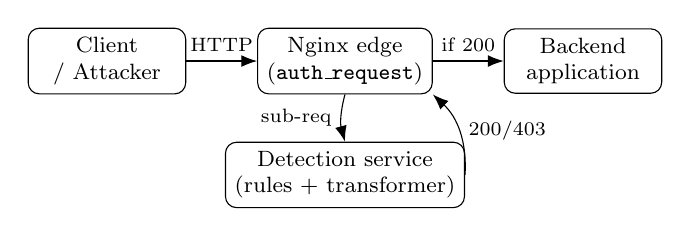
\begin{tikzpicture}[
  node distance=6mm and 9mm,
  box/.style={draw,rounded corners,align=center,minimum height=8mm,
              minimum width=20mm,font=\footnotesize},
  every edge/.style={draw,-{Latex[length=2mm]}}]
  \node[box] (client) {Client\\/ Attacker};
  \node[box,right=of client] (nginx) {Nginx edge\\(\texttt{auth\_request})};
  \node[box,below=of nginx] (waf) {Detection service\\(rules + transformer)};
  \node[box,right=of nginx] (app) {Backend\\application};
  \draw (client) edge node[above,font=\scriptsize]{HTTP} (nginx);
  \draw (nginx.south) edge[bend right=15] node[left,font=\scriptsize]{sub-req} (waf.north);
  \draw (waf.east) edge[bend right=25] node[right,font=\scriptsize]{200/403} (nginx.south east);
  \draw (nginx) edge node[above,font=\scriptsize]{if 200} (app);
\end{tikzpicture}
\caption{Inline enforcement. Every request is adjudicated by the detection
service through Nginx \texttt{auth\_request} before it can reach the backend.}
\label{fig:arch}
\end{figure}

\subsection{Four-tier detection pipeline}
Inside the detection service a request passes through four tiers of increasing
cost and decreasing certainty (Fig.~\ref{fig:flow}). Tier~1 matches a small set
of unambiguous signatures (for example \texttt{or 1=1}, \texttt{union select},
\texttt{<script}, \texttt{../}) after double URL-decoding, and blocks on a
match. Tier~2 applies anomaly and injection rules: a suspicious-keyword lexicon,
encoding-abuse patterns, injection regular expressions, and a special-character
density threshold. Tier~3 invokes the transformer, which scores the normalised
request and returns a malicious probability. Tier~4 fuses these signals into a
final decision, described formally in Section~\ref{sec:method}. Two policies
modulate the pipeline: safe internal endpoints (static assets, real-time
channels) are evaluated only against Tier~1 to protect legitimate high-volume
traffic from model uncertainty, and any unhandled error in the path fails open,
trading a missed detection for availability.

\begin{figure}[t]
\centering
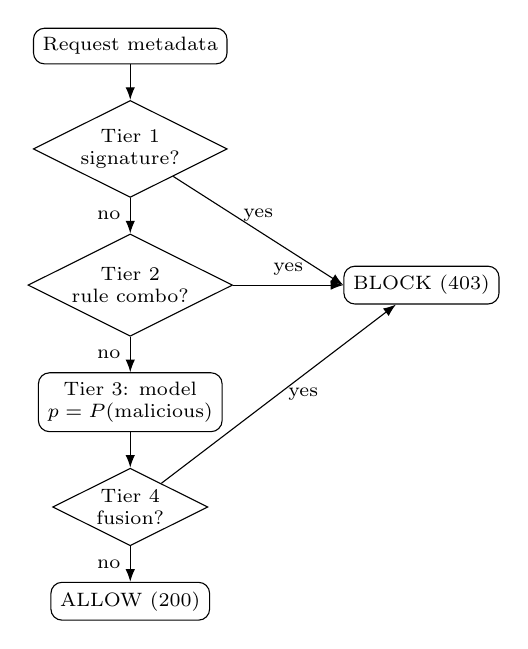
\begin{tikzpicture}[
  node distance=4.5mm,
  dec/.style={draw,diamond,aspect=2,align=center,font=\scriptsize,inner sep=1pt},
  act/.style={draw,rounded corners,align=center,font=\scriptsize,minimum width=16mm},
  every edge/.style={draw,-{Latex[length=1.6mm]}}]
  \node[act] (in) {Request metadata};
  \node[dec,below=of in] (t1) {Tier 1\\signature?};
  \node[dec,below=of t1] (t2) {Tier 2\\rule combo?};
  \node[act,below=of t2] (t3) {Tier 3: model\\$p=P(\text{malicious})$};
  \node[dec,below=of t3] (t4) {Tier 4\\fusion?};
  \node[act,right=14mm of t2] (block) {BLOCK (403)};
  \node[act,below=of t4] (allow) {ALLOW (200)};
  \draw (in) edge (t1);
  \draw (t1) edge node[left,font=\scriptsize]{no} (t2);
  \draw (t1) edge node[above,font=\scriptsize]{yes} (block.west);
  \draw (t2) edge node[above,font=\scriptsize]{yes} (block);
  \draw (t2) edge node[left,font=\scriptsize]{no} (t3);
  \draw (t3) edge (t4);
  \draw (t4) edge node[right,font=\scriptsize]{yes} (block);
  \draw (t4) edge node[left,font=\scriptsize]{no} (allow);
\end{tikzpicture}
\caption{Decision flow. Cheap deterministic tiers short-circuit obvious cases;
the transformer and fusion tier adjudicate the ambiguous remainder.}
\label{fig:flow}
\end{figure}

%=======================================================================
\section{Methodology}
\label{sec:method}

\subsection{Problem formulation}
We treat detection as binary classification of an HTTP request into benign
($0$) or malicious ($1$). Each request is reduced to a text string
$x = \texttt{METHOD}\;\Vert\;\texttt{URI}'$, where $\texttt{URI}'$ is the
request path and query after normalisation. A classifier estimates
$p = P(y{=}1 \mid x)$, and the fusion policy maps $p$ together with rule signals
to a decision.

\subsection{Datasets}
We use \ph{N} public corpora (Table~\ref{tab:datasets}).
CSIC~2010~\cite{gimenez2010csic} provides the standard benchmark and enables
comparison with prior work; a second corpus
(ECML/PKDD~2007~\cite{pkdd2007} or SR-BH~\cite{srbh2020}) supplies an
independent distribution for the cross-dataset protocol. Each corpus is parsed
into the unified schema, deduplicated, and split $70/15/15$ into
train/validation/test with stratification on the label and a fixed random seed.

\begin{table}[t]
\centering
\caption{Datasets after preprocessing. Fill counts from
\texttt{prepare\_datasets.py} output.}
\label{tab:datasets}
\begin{tabular}{@{}lcccc@{}}
\toprule
Dataset & Benign & Malicious & Total & Malicious \% \\
\midrule
CSIC 2010 & \ph{n} & \ph{n} & \ph{n} & \ph{\%} \\
\ph{Second set} & \ph{n} & \ph{n} & \ph{n} & \ph{\%} \\
\bottomrule
\end{tabular}
\end{table}

\subsection{Preprocessing and tokenisation}
The request is double URL-decoded to expose encoded payloads, contiguous digit
runs are replaced by a single placeholder token to prevent the model from
overfitting to identifiers, and the \texttt{METHOD URI} string is tokenised with
the base model's WordPiece vocabulary at a maximum length of $256$ tokens. The
same preprocessing is applied at training and inference time and is shared with
the deployed service.

\subsection{Model}
The classifier is a pretrained transformer encoder with a dropout layer and a
linear head over the pooled \texttt{[CLS]} representation, fine-tuned end to end
for binary classification. To test whether domain pretraining helps HTTP request
classification, we fine-tune three interchangeable base encoders under identical
settings: \texttt{bert-base-uncased}~\cite{devlin2019bert} as a general-language
baseline, SecureBERT~\cite{aghaei2022securebert} as a cybersecurity-pretrained
encoder, and DistilBERT~\cite{sanh2019distilbert} as a latency-oriented
variant. Optimisation uses AdamW with a warmup schedule, weight decay, and early
stopping on validation F1.

\subsection{Decision fusion}
The fusion tier (Algorithm~\ref{alg:fusion}) blocks on an unambiguous signature,
then on a keyword--injection combination or an encoding attack, and only then
consults the model. Crucially, the model never blocks alone: a request is
blocked on model evidence only when a high-confidence score coincides with an
independent rule signal, or when a score in the uncertainty band coincides with a
keyword or character anomaly. This coupling is the mechanism by which the design
bounds false positives---an isolated high model score on otherwise clean traffic
does not cause a block.

\begin{algorithm}[t]
\caption{Decision fusion (Tier 4)}
\label{alg:fusion}
\begin{algorithmic}[1]
\Require request $(\text{method},\text{uri})$, model score $p$, thresholds
$\tau_h{=}0.98$, $\tau_\ell{=}0.90$
\State $u \gets \text{doubleDecode}(\text{uri})$
\If{$\text{directSignature}(u)$} \Return \textsc{block}, $1.0$ \EndIf
\State $s \gets \text{ruleSignals}(u)$
\If{$s.\text{keyword} \wedge s.\text{injection}$} \Return \textsc{block} \EndIf
\If{$s.\text{encoding}$} \Return \textsc{block} \EndIf
\If{$p > \tau_h \wedge s.\text{hasSignal}$} \Return \textsc{block}, $p$ \EndIf
\If{$\tau_\ell \le p < \tau_h \wedge (s.\text{keyword} \vee s.\text{charAnom})$}
   \Return \textsc{block}, $p$ \EndIf
\State \Return \textsc{allow}, $p$
\end{algorithmic}
\end{algorithm}

%=======================================================================
\section{Experimental Setup}
\label{sec:setup}
\textbf{Metrics.} We report accuracy, precision, recall, F1, false-positive rate
(FPR) and ROC--AUC, and per-attack-class recall. We emphasise FPR because the
operational cost of a WAF is dominated by wrongly blocking legitimate users.

\textbf{Baselines.} We compare against (i) the deterministic rule engine alone
(Tier~1--2), (ii) TF--IDF character $n$-gram features with a linear SVM, a random
forest and logistic regression, and (iii) published transformer results on
CSIC~2010 cited from the literature.

\textbf{Protocols.} \emph{Within-dataset}: train and test on the same corpus's
splits. \emph{Cross-dataset}: train on one corpus, test on another corpus's held
test split, to measure transfer to an unseen distribution. \emph{Ablation}:
evaluate rules-only, model-only and the full hybrid on the same test set.
\emph{Threshold sensitivity}: sweep the decision threshold and record the
FPR/recall trade-off. \emph{Latency}: measure per-request model inference on CPU
and GPU, and end-to-end request latency through the live stack under concurrent
load.

\textbf{Environment.} \ph{CPU/GPU model}, \ph{RAM}, PyTorch~\ph{ver},
Transformers~\ph{ver}, Docker~\ph{ver}. All seeds fixed to $42$.

%=======================================================================
\section{Results}
\label{sec:results}
\emph{The tables below are structured for your results; replace every red
placeholder with the numbers emitted by the \texttt{research/} scripts.}

\subsection{Detection quality and baselines}
Table~\ref{tab:main} reports within-dataset detection for every model against
the baselines. \ph{One or two sentences stating the headline F1/FPR of the
hybrid and how it compares to rules-only and classical ML.}

\begin{table}[t]
\centering
\caption{Within-dataset detection on CSIC 2010 (test split).}
\label{tab:main}
\begin{tabular}{@{}lccccc@{}}
\toprule
Method & P & R & F1 & FPR & AUC \\
\midrule
Rule engine only          & \ph{} & \ph{} & \ph{} & \ph{} & --- \\
TF--IDF + LinearSVM       & \ph{} & \ph{} & \ph{} & \ph{} & \ph{} \\
TF--IDF + RandomForest    & \ph{} & \ph{} & \ph{} & \ph{} & \ph{} \\
BERT (model only)         & \ph{} & \ph{} & \ph{} & \ph{} & \ph{} \\
SecureBERT (model only)   & \ph{} & \ph{} & \ph{} & \ph{} & \ph{} \\
DistilBERT (model only)   & \ph{} & \ph{} & \ph{} & \ph{} & \ph{} \\
\textbf{Hybrid (ours)}    & \ph{} & \ph{} & \ph{} & \ph{} & \ph{} \\
\bottomrule
\end{tabular}
\end{table}

\subsection{Ablation: does the transformer earn its cost?}
Table~\ref{tab:ablation} isolates each layer. \ph{State whether the hybrid
exceeds both rules-only and model-only, and by how much; if the rules already
catch most attacks, say so honestly and quantify the model's marginal
contribution.}

\begin{table}[t]
\centering
\caption{Ablation on the same test set.}
\label{tab:ablation}
\begin{tabular}{@{}lcccc@{}}
\toprule
Configuration & P & R & F1 & FPR \\
\midrule
Rules only  & \ph{} & \ph{} & \ph{} & \ph{} \\
Model only  & \ph{} & \ph{} & \ph{} & \ph{} \\
Hybrid      & \ph{} & \ph{} & \ph{} & \ph{} \\
\bottomrule
\end{tabular}
\end{table}

\subsection{Cross-dataset generalisation}
Table~\ref{tab:cross} reports transfer to an unseen corpus. Some degradation is
expected; \ph{report the retained F1 and analyse which attack classes transfer
and which do not.}

\begin{table}[t]
\centering
\caption{Cross-dataset transfer (train $\rightarrow$ test).}
\label{tab:cross}
\begin{tabular}{@{}lcccc@{}}
\toprule
Train $\rightarrow$ Test & P & R & F1 & FPR \\
\midrule
CSIC $\rightarrow$ CSIC (ref.) & \ph{} & \ph{} & \ph{} & \ph{} \\
CSIC $\rightarrow$ \ph{other}  & \ph{} & \ph{} & \ph{} & \ph{} \\
\ph{other} $\rightarrow$ CSIC  & \ph{} & \ph{} & \ph{} & \ph{} \\
\bottomrule
\end{tabular}
\end{table}

\subsection{Threshold sensitivity and false-positive control}
Fig.~\ref{fig:threshold} plots FPR and recall as the decision threshold varies;
the chosen operating point \ph{value} yields FPR~\ph{} at recall~\ph{}. \ph{One
sentence justifying the operating point.}

\begin{figure}[t]
\centering
% Replace with a plot of results/threshold_*.csv (e.g. via pgfplots or an
% exported PDF from matplotlib). Placeholder box shown below.
\fbox{\parbox[c][32mm][c]{0.9\columnwidth}{\centering\footnotesize
\ph{Insert threshold-sweep figure from results/threshold\_csic.csv}
(x: threshold, y: FPR and recall)}}
\caption{False-positive/recall trade-off versus decision threshold.}
\label{fig:threshold}
\end{figure}

\subsection{Latency and throughput}
Table~\ref{tab:latency} reports inline overhead. \ph{State median and p99
per-request latency and sustained throughput, and contrast the DistilBERT
variant against the full model.}

\begin{table}[t]
\centering
\caption{Per-request latency and throughput.}
\label{tab:latency}
\begin{tabular}{@{}lcccc@{}}
\toprule
Configuration & p50 (ms) & p95 (ms) & p99 (ms) & RPS \\
\midrule
Nginx only (no WAF)      & \ph{} & \ph{} & \ph{} & \ph{} \\
+ rules                  & \ph{} & \ph{} & \ph{} & \ph{} \\
+ BERT (CPU)             & \ph{} & \ph{} & \ph{} & \ph{} \\
+ BERT (GPU)             & \ph{} & \ph{} & \ph{} & \ph{} \\
+ DistilBERT             & \ph{} & \ph{} & \ph{} & \ph{} \\
\bottomrule
\end{tabular}
\end{table}

\subsection{Adversarial evasion}
Table~\ref{tab:adv} reports the fraction of initially blocked payloads that
evade detection after each semantics-preserving mutation. \ph{Report the overall
evasion rate and identify the most effective mutation; discuss implications for
robustness.}

\begin{table}[t]
\centering
\caption{Evasion rate under semantics-preserving mutation.}
\label{tab:adv}
\begin{tabular}{@{}lc@{}}
\toprule
Mutation & Evasion rate \\
\midrule
Inline comment      & \ph{} \\
Case randomisation  & \ph{} \\
URL encoding        & \ph{} \\
Double encoding     & \ph{} \\
Whitespace/tab      & \ph{} \\
Junk parameter      & \ph{} \\
\textbf{Overall}    & \ph{} \\
\bottomrule
\end{tabular}
\end{table}

%=======================================================================
\section{Discussion and Limitations}
\label{sec:discussion}
The fail-open safeguard trades security for availability, and its activation
frequency \ph{report it} bounds the exposure this introduces. The detector
inspects the request line and, where available, the request body; response
traffic is not analysed, so exfiltration in responses is out of scope, and we
make no such claim. The adversarial results \ph{summarise} indicate that
semantics-preserving mutation remains a threat, consistent with
WAF-A-MoLE~\cite{demetrio2020wafamole}; adversarial training is a natural
extension. Safe online adaptation to concept drift is deliberately excluded:
naively treating allowed traffic as benign is a label-poisoning risk, and a
human-in-the-loop or verified-feedback design is required. Finally, the
evaluation is single-backend and does not cover distributed deployment.

%=======================================================================
\section{Conclusion}
\label{sec:conclusion}
We presented a web application firewall that places a fine-tuned transformer in a
transparent inline enforcement path and governs it with a false-positive-aware
rule--model fusion policy. Unlike the offline transformer-WAF literature, we
characterised the system end to end: detection quality with an emphasis on
false-positive rate, an ablation isolating the model's contribution,
cross-dataset generalisation, threshold sensitivity, measured inline latency, and
adversarial evasion. \ph{Close with the headline result once filled.} Future work
includes distillation and quantisation for lower latency, request-body and
response inspection, adversarial training, and verified online adaptation.

%=======================================================================
\bibliographystyle{IEEEtran}
\bibliography{../references}

\end{document}
